\documentclass{beamer}

\usepackage{textcomp}
\usepackage{xcolor}
\usepackage{listings}
\usepackage{matlab-prettifier}
\usepackage[T1]{fontenc}
\usepackage{multimedia}
\usepackage{hyperref}

\usepackage{caption}
\captionsetup{justification=raggedright,singlelinecheck=false}

\usetheme{Boadilla}

\makeatletter
\def\blfootnote{\gdef\@thefnmark{}\@footnotetext}
\makeatother
\urlstyle{sf}

\title{Crabsort}
\subtitle{Spike-sorting for small circuit networks}
\author{Alec Hoyland & Cosmo Guerini}
\institute[CSN]{Center for Systems Neuroscience}

\begin{document}

%% title page

\begin{frame}
  \titlepage
\end{frame}


\section{Introduction}

\begin{frame}
  \frametitle{Spike-sorting primer}

  Spike-sorting is the process of mapping action potentials to the originating cell.

  \begin{columns}
    \column{0.5\textwidth}

    \begin{figure}
      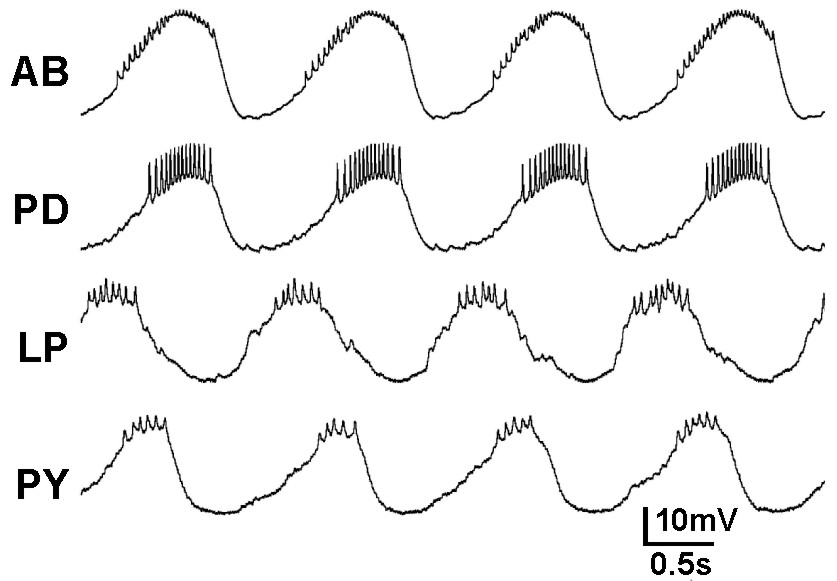
\includegraphics[width=\textwidth]{gfx/pyloric.jpeg}
      \centering
      \caption{Intracellular recordings of pyloric cells.}
      \label{fig:intracellular}
    \end{figure}

    \column{0.5\textwidth}

    \begin{figure}
      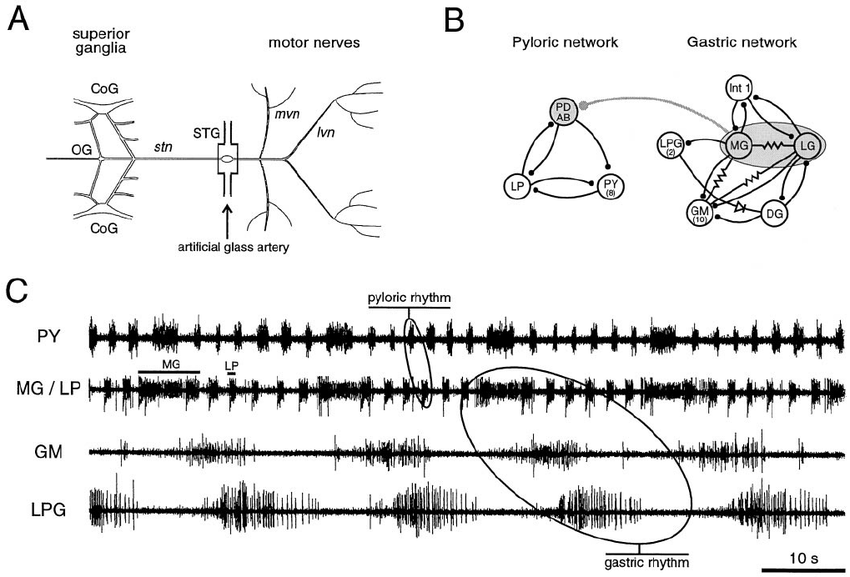
\includegraphics[width=\textwidth]{gfx/STG-rhythms.png}
      \centering
      \caption{\textbf{A} circuit diagram of nerves; \textbf{B} connectivity diagram, circles are cells, synapses are lines and dots; \textbf{C} extracellular recording of motor nerves.}
      \label{fig:extracellular}
    \end{figure}

  \end{columns}

\end{frame}

% \subsection{Rationale}
%
% %% Design Principles
%
% \begin{frame}
%   \frametitle{Design Principles}
%
%   \begin{columns}
%     \column{0.5\textwidth}
%
%     Xolotl should be
%
%     \begin{itemize}
%       \item fast
%       \item easy-to-use
%       \item well-documented
%       \item hackable and extensible
%       \item auditable
%     \end{itemize}
%
%     \column{0.5\textwidth}
%
%     \includegraphics[width=\textwidth]{gfx/fast.png}
%     \centering
%
%     \includegraphics[width=\textwidth]{gfx/documentation.png}
%     \centering
%
%   \end{columns}
%
% \end{frame}
%
% \subsection{Design}
%
% %% How Xolotl Works
%
% \begin{frame}
%   \frametitle{How xolotl works}
%
%   \begin{figure}
%     \includegraphics[width=\textwidth]{gfx/fig1.jpg}
%     \caption{Model of A \& B represented in code C which produces D-I.}
%   \end{figure}
%
% \end{frame}
%
% %% Anatomy of a Model
%
% \begin{frame}[fragile]
%   \frametitle{Anatomy of a model}
%
%   \begin{columns}
%
%     \column{0.35\textwidth}
%     Types of Components:
%
%     \begin{itemize}
%       \item Compartments
%       \begin{itemize}
%         \item Mechanisms
%       \end{itemize}
%       \begin{itemize}
%         \item Conductances
%         \begin{itemize}
%           \item Mechanisms
%         \end{itemize}
%         \item Synapses
%         \begin{itemize}
%           \item Mechanisms
%         \end{itemize}
%       \end{itemize}
%     \end{itemize}
%
%
%     \begin{figure}
%       \includegraphics[width=\textwidth]{gfx/liu.png}
%       \centering
%       \caption{100+ components are a searchable, indexed feature of the language.}
%     \end{figure}
%
%     \column{0.65\textwidth}
%
%     Code to generate an HH model with constant injected current:
%
%     \resizebox{\textwidth}{!}{\lstinputlisting[style=Matlab-editor,breaklines=false]{code/HH.m}}
%
%   \end{columns}
%
% \end{frame}
%
% \subsection{Features}
%
% %% Cool Features
%
% \begin{frame}{Embedded Animation}
%   \frametitle{Cool features}
%
%     \begin{itemize}
%       \item \texttt{puppeteer}: real-time parameter manipulation
%       \item \texttt{xgrid}: parallel simulation across a distributed network
%       \item \texttt{xfit}: parameter optimization using particle swarm and genetic algorithms
%       \item \texttt{xtools}: spike counting and data analysis
%       \item model hashing and snapshotting
%       \item control over input and output (clamping, full state matrix)
%       \item automatic component generation from MATLAB
%       \item hyperlinking and tab-completion in the console
%       \item multiple solvers, look-up table caching
%     \end{itemize}
%
% \end{frame}
%
% %% Coming Soon
%
% \begin{frame}{Embedded Animation}
%   \frametitle{Coming Soon}
%
%     \begin{itemize}
%       \item multi-threading of a single simulation
%       \item server-side compilation / stand-alone integration
%       \item (multi-compartment) server-side GPU computation of Hines matrices
%       \item new compartment types (including low-dimensional models)
%       \item universal support for Runge-Kutta integration schemes
%       \item adaptive time-step solvers (quadrature)
%       \item robust front-end unit support
%       \item Julia front-end (compatible with Python, etc.)
%     \end{itemize}
%
% \end{frame}
%
% %% Pretty Plots
%
% \begin{frame}
%   \frametitle{Real-time manipulation}
%
%     \begin{center}
%       \movie[width=\textwidth, height=0.3\textwidth, loop]{}{gfx/manipulate-neuron.mp4}
%       \caption{Real-time parameter manipulation. Any numerical xolotl property can be manipulated.}
%     \end{center}
%
% \end{frame}
%
% \begin{frame}
%   \frametitle{\texttt{xfit}: Parameter optimization}
%
%   \begin{columns}
%     \column{0.5\textwidth}
%     Optimized for:
%
%     \begin{enumerate}
%       \item Slow-wave troughs at -70 mV.
%       \item Slow-wave peaks at -40 mV.
%       \item Spike downswing ends above slow wave trough.
%       \item Burst frequency of 0.5 Hz.
%       \item Duty cycle of 0.3.
%     \end{enumerate}
%
%     \column{0.5\textwidth}
%     \begin{figure}
%       \includegraphics[width=\textwidth]{gfx/xfit.png}
%       \centering
%       \caption{Fit of 8-conductance model (left to right). PSO \#2 shown.}
%     \end{figure}
%   \end{columns}
%
% \end{frame}
%
% \section{Demonstrations}
%
% \subsection{Installing}
%
% %% Getting Started
%
% \begin{frame}[fragile]
%   \frametitle{Installing}
%
%   Acquiring the MATLAB toolbox
%   \medskip
%
%   \begin{enumerate}
%     \item Go to \url{https://github.com/sg-s/xolotl/releases/latest}
%     \item Download \texttt{xolotl.mltbox}
%     \item Find the file in \texttt{Downloads} and drag it onto your \texttt{MATLAB} workspace
%           This will install \texttt{xolotl}
%   \end{enumerate}
%
%   \blfootnote{\url{https://xolotl.readthedocs.io/en/master/tutorials/start-here/}}
%
% \end{frame}
%
% %% Setup in MATLAB
%
% \begin{frame}[fragile]
%
%   Run the following commands in MATLAB. You should see this plot.
%
%   \resizebox{0.5\textwidth}{!}{\lstinputlisting[style=Matlab-editor,breaklines=false]{code/setup.m}}
%   \medskip
%
%   \begin{figure}
%     \includegraphics[width=\textwidth]{gfx/demo_bursting_neuron.png}
%   \end{figure}
%
%   \blfootnote{\url{https://xolotl.readthedocs.io/en/master/tutorials/built-in-demos/}}
%
% \end{frame}
%
% %% Demos
%
% \subsection{Demonstrations}
%
% \begin{frame}
%   \frametitle{Demonstrations}
%
%   Your first neuron
%
%   \medskip
%
%   \url{https://xolotl.readthedocs.io/en/master/tutorials/first-neuron/}
%
%   \medskip
%   Your first network
%   \medskip
%
%   \url{https://xolotl.readthedocs.io/en/master/tutorials/first-network/}
%
%   \medskip
%   All demos
%   \medskip
%
%   \url{https://xolotl.readthedocs.io/en/master/tutorials/built-in-demos/}\medskip
%
% \end{frame}


\end{document}
